\documentclass[11pt,letterpaper]{article}
\usepackage[margin=1in]{geometry}
\usepackage{graphicx}
\usepackage{hyperref}
\usepackage{listings}
\usepackage{amsmath}
\pagestyle{headings}
\usepackage{epstopdf}

\begin{document}

\title{PHY 410 \\ Homework Assignment 5}
\author{Han Wen \\ \tiny Person No. 50096432}
\date{\today}

\maketitle

\begin{abstract}
The goal of this assignment was to get familiar with the numerical method in linear algebra. Including solving the problems related to resistance of a system and the normal mode problem. 


\end{abstract}

\tableofcontents

\newpage
\section{Problem 1}

\subsection{Description}
Resistor Cube: Write a program to solve for the currents in a resistor cube. There are 12 resistors, one along each edge. A voltage source is connected across a body diagonal of the cube. To analysis this problem we will denote the current in each resistor with the same number of the resistor itself. However, all 12 currents are not completely independent, only 6 out of 12 are. 

    Find the equivalent resistance for the symmetric case when all the resistors have the same resistance, say 1 Ohm. You might remember this problem from freshman EM.
    Plot the equivalent resistance as a function of one resistor (choose any one) when all 11 others are fixed at 1 Ohm
    How many different cases are there when one resistor is varied as in the previous part?





\subsection{Numerical Analysis}

To solve this problem we are going to use Kirchoff's Law and solve the matrix equation. Here is a diagram showing the resistor cube ~\ref{figure1}. 
To be specific, here is a table denoting all 12 currents with 6 of them: \ref{table1}

\begin{table}[h]
\caption{currents\label{table1}}
\begin{tabular}{l l}
\hline
 \textbf{current } & \textbf{represent}\\
\hline
$I_1$ & $I_1$ \\
$I_2$ & $I_2$ \\
$I_3$ & $I_3$ \\
$I_4$ & $I_4$ \\
$I_5$ & $I_5$ \\
$I_6$ & $I_1-I_2+I_5$ \\
$I_7$ & $I_9-I_5+I_4-I_3$ \\
$I_8$ & $I_9-I_5$ \\
$I_9$ & $I_9$ \\
$I_{10}$ & $I_1-I_2$ \\
$I_{11}$ & $I_2+I_3$ \\
$I_{12}$ & $I_4-I_3$ \\
\hline
\end{tabular}
\end{table}

Then, we can use Kirchoff's law to make equations:

\[
  \begin{cases}
   -R_7I_3+R_7I_4-(R_7+R_8)I_5+(R_9+R_8)I_9=V \\
   R_6I_1-R_6I_2+(R_6+R_9)I_5+R_9I_9=V\\
   (R_1+R_{10}+R_6)I_1-(R_{10}+R_6)I_2+R_6I_5=V\\
   R_1I_1+(R_2+R_1)I_2+R_{11}I_3=V\\
   R_{11}I_2+(R_3+R_{11})I_3+R_4I_4=V\\
   -(R_{12}+R_7)I_3+(R_4+R_{12}+R_7)I_4-R_7I_5+R_7I_9=V
  \end{cases}
\]

And consequently the matrix equation can be expressed as:
$$
\begin{pmatrix}
 0 & 0 & -R_7 & R_7 & -(R_7+R_8) & (R_8+R_9) \\
 R_6 & -R_6 & 0 & 0 & (R_6+R_9) & R_9 \\
 (R_1+R_6+R_{10}) & -(R_6+R_{10}) & 0 & 0 & R_6 & 0\\
 R_1 & (R_2+R_{11}) & R_{11} & 0 & 0 & 0 \\
 0 & R_{11} & (R_3+R_{11}) & R_4 & 0 & 0 \\
 0 & 0 & -(R_{12}+R_7) & (R_4+R_{12}+R_7) & -R_7 & R_7 
\end{pmatrix}
\begin{pmatrix}
 I_1\\
 I_2\\
 I_3\\
 I_4\\
 I_5\\
 I_9
\end{pmatrix}
=
\begin{pmatrix}
 V\\
 V\\
 V\\
 V\\
 V\\
 V
\end{pmatrix}
$$
Solving this matrix equation and use $I_0=I_1+I_4+I_9$, combine with $R_{total}=\frac{V}{I_0}$ we can calculate the total resistance.

\subsection{Result}

For part 1, if all the resistances are 1 Ohm, then my result is the total resistance is 0.833 Ohm, same with the analytical solution.

For part 2 and 3, we can see due to the symmetry in this system, only two different cases. One is varying $R_1,R_4,R_9,R_6,R_7,R_{11}$ another is varying the rest of the resistors resistances. In my diagram, the blue one stands for the first case, and the green one stands for the second. ~\ref{figure2}

 
\begin{figure}
\begin{center}
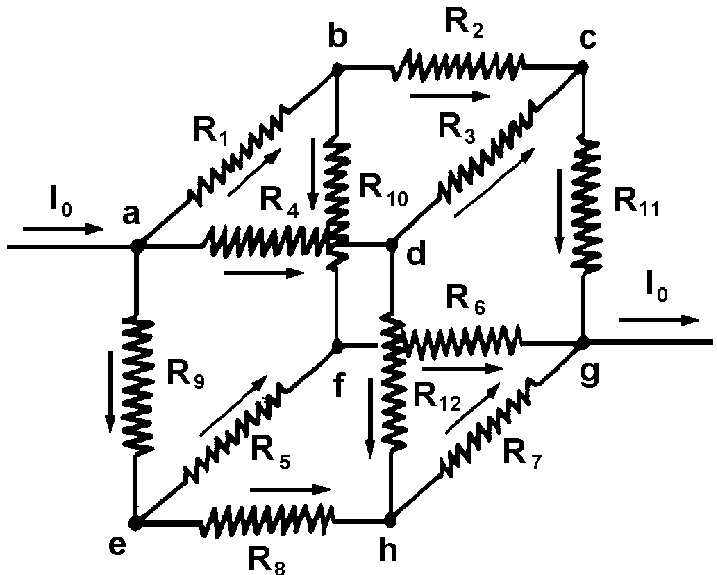
\includegraphics[width=0.6\linewidth,angle=0]{cube.png}
\caption{Resistor cube}
\label{figure1}
\end{center}
\end{figure}

\begin{figure}
\begin{center}
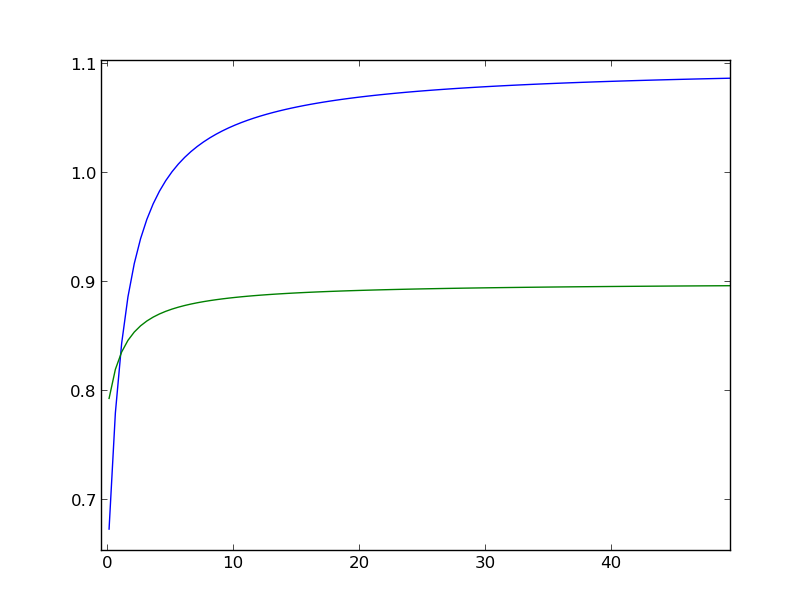
\includegraphics[width=0.6\linewidth,angle=0]{p1.png}
\caption{Resistor cube varying one resistor}
\label{figure2}
\end{center}
\end{figure}



\newpage

\section{Problem 2}

\subsection{Description}
  Carbon suboxide is five-atom linear molecule. Simulate a   molecule with a linear system of 5 masses and 4 ideal springs, similar to the linear triatomic molecule. There are two distinct mass values   and  , and two distinct force constants   and  . Search the web for information on the force constants. If you cannot locate data on  , make a reasonable estimate from data on Molecular Vibrations simpler molecules with similar bonds, for example CO2). Find the eigenfrequencies and normal modes for longitudinal oscillations.

\subsection{Analysis}
I found the bond strength for C=C and C=O bond are:960N/m and 1210N/m \cite{bond}. As we can see the structure of the carbon suboxide is that five atoms are linearly arranged with two oxygen atoms at two sides and three carbon atoms in the middle. If denoted by $x_1$ to $x_5$, the spring constant of C=C with $K_{cc}$ and that of C=O with $K_{co}$, mass of oxygen and carbon as M and m, then we have:
\[
  \begin{cases}
	M\ddot{x_1}=-K_{co}x_1+K_{co}x_2\\
	m\ddot{x_2}=K_{co}x_1-(K_{co}+K_{cc})x_2+K_{cc}x_3\\
	m\ddot{x_3}=K_{cc}x_2-2K_{cc}x_3+K_{cc}x_4\\
	m\ddot{x_4}=K_{cc}x_3-(K_{co}+K_{cc})x_4+K_{co}x_5\\
	M\ddot{x_5}=K_{co}x_4-K_{co}x_5\\
  \end{cases}
\]

Written in matrix form:
$$
\begin{pmatrix}
 -K_{co} & K_{co} & 0 & 0 & 0 \\
 K_{co} & -(K_{co}+K_{cc}) & K_{cc} & 0 & 0 \\
 0 & K_{cc} & -2K_{cc} & K_{cc} & 0 \\
 0 & 0 & K_{cc} & -(K_{co}+K_{cc}) & K_{co} \\
 0 & 0 & 0 & K_{co} & -K_{co} 
\end{pmatrix}
\begin{pmatrix}
 x_1\\
 x_2\\
 x_3\\
 x_4\\
 x_5
\end{pmatrix}
=
\begin{pmatrix}
 M & 0 & 0 & 0 & 0\\
 0 & m & 0 & 0 & 0\\
 0 & 0 & m & 0 & 0\\
 0 & 0 & 0 & m & 0\\
 0 & 0 & 0 & 0 & M
\end{pmatrix}
\begin{pmatrix}
 \ddot{x_1}\\
 \ddot{x_2}\\
 \ddot{x_3}\\
 \ddot{x_4}\\
 \ddot{x_5}
\end{pmatrix}
$$

With the normal mode method, it becomes:

$$
\begin{pmatrix}
 K_{co} & -K_{co} & 0 & 0 & 0 \\
 -K_{co} & (K_{co}+K_{cc}) & -K_{cc} & 0 & 0 \\
 0 & -K_{cc} & 2K_{cc} & -K_{cc} & 0 \\
 0 & 0 & -K_{cc} & (K_{co}+K_{cc}) & -K_{co} \\
 0 & 0 & 0 & -K_{co} & K_{co} 
\end{pmatrix}
\begin{pmatrix}
 x_1\\
 x_2\\
 x_3\\
 x_4\\
 x_5
\end{pmatrix}
=\omega^2
\begin{pmatrix}
 M & 0 & 0 & 0 & 0\\
 0 & m & 0 & 0 & 0\\
 0 & 0 & m & 0 & 0\\
 0 & 0 & 0 & m & 0\\
 0 & 0 & 0 & 0 & M
\end{pmatrix}
\begin{pmatrix}
 x_1\\
 x_2\\
 x_3\\
 x_4\\
 x_5
\end{pmatrix}
$$

to simplify the problem, we let m=12 and M=16, $K_{cc}=0.96$ and $K_{co}=1.21$.


\subsection{Result}
Thus I found the eigenfrequencies:
$$
\omega^2=
\begin{pmatrix}
 0.02628\\
 0\\
 0.11296\\
 0.23017\\
 0.30350
\end{pmatrix}
$$

and the corresponding eigenvectors are:
$$
\begin{pmatrix}
 -0.15 & -0.12 & 0.12 & 0.09 & 0.05\\
 -0.10 & -0.12 & -0.06 & -0.18 & -0.15\\
 0.00 & -0.12 & -0.20 & 0.00 & 0.17\\
 0.10 & -0.12 & -0.06 & 0.18 & -0.15\\
 0.15 & -0.12 & 0.12 & -0.09 & 0.05
\end{pmatrix}
$$



\newpage

\section{Problem 3}
\subsection{Description}
(a) Repeat Problem 1 for an octahedron instead of a cube. Describe any similarities or differences in your solutions. 
(b) Solve Problem 2 analytically (see e.g. Goldstein, Poole and Safko Problem 6.6) and compare with your numerical solution.

\subsection{Result}

(a) As shown in the figure, we denote from top to bottom from 1 to 12 ~\ref{figure3}. Similarly we choose 8 independent variables to solve the problem this time(Though we can take advantage of the symmetric property to reduce the degree of freedom, I believe a more general solution is more elegant here, in spite of the greater difficulty):

\begin{table}[h]
\caption{currents of octahedron\label{table2}}
\begin{tabular}{l l}
\hline
 \textbf{current} & \textbf{represent}\\
\hline
$I_1$ & $I_1$ \\
$I_2$ & $I_2$ \\
$I_3$ & $I_3$ \\
$I_4$ & $I_4$ \\
$I_5$ & $I_5$ \\
$I_6$ & $I_6$ \\
$I_7$ & $I_7$ \\
$I_8$ & $I_8$ \\
$I_9$ & $I_1+I_5-I_6$ \\
$I_{10}$ & $I_2+I_6-I_7$  \\
$I_{11}$ & $I_3+I_7-I_8$  \\
$I_{12}$ & $I_4+I_8-I_5$  \\
\hline
\end{tabular}
\end{table}

Therefore the matrix equation is :
$$
\begin{pmatrix}
 (R_1+R_9) & 0 & 0 & 0 & R_9 & -R_9 & 0 & 0   \\
 0 & (R_2+R_{10}) & 0 & 0 & 0 & R_{10} & -R_{10} & 0 \\
 0 & 0 & (R_3+R_{11}) & 0 & 0 & 0 & R_{11} & -R_{11} \\
 0 & 0 & 0 & (R_4+R_{12}) & -R_{12} & 0 & 0 & R_{12} \\
 R_1 & -R_2 & 0 & 0 & 0 & R_6 & 0 & 0 \\
 0 & R_2 & -R_3 & 0 & 0 & 0 & R_7 & 0 \\
 0 & 0 & R_3 & -R_4 & 0 & 0 & 0 & R_8 \\
 -R_1 & 0 & 0 & R_4 & R_5 & 0 & 0 & 0 
\end{pmatrix}
\begin{pmatrix}
 I_1\\
 I_2\\
 I_3\\
 I_4\\
 I_5\\
 I_6\\
 I_7\\
 I_8\\
\end{pmatrix}
=
\begin{pmatrix}
 V\\
 V\\
 V\\
 V\\
 0\\
 0\\
 0\\
 0
\end{pmatrix}
$$

When all the resistances are 1 Ohm, the total resistance is 0.5 Ohm, same with the theoretical value.

Similar to the previous system, still only two cases exist. One is changing $R_5.R_6,R_7,R_8$ another is changing other resistors.
However, considering when all $R_1-R_4 and R_9-R_{12}$ are equal to each other, the variation of $R_5-R_8$ won't change the result.

Here is a diagram showing the relationship between the total resistance and the change of one resistor. The green line stands for $R_1$ changing. The blue line stands for when the aforementioned 8 resistors are not equal, the $R_5$ changing case. ~\ref{figure4} 

\newpage
\begin{figure}
\begin{center}
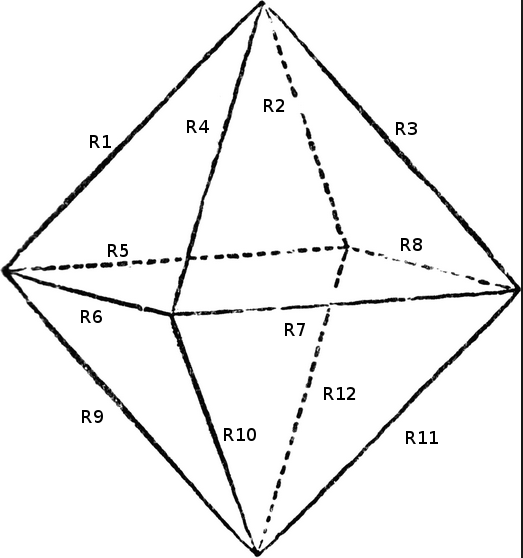
\includegraphics[width=0.6\linewidth,angle=0]{oc.png}
\caption{Octahedron}
\label{figure3}
\end{center}
\end{figure}


\begin{figure}
\begin{center}
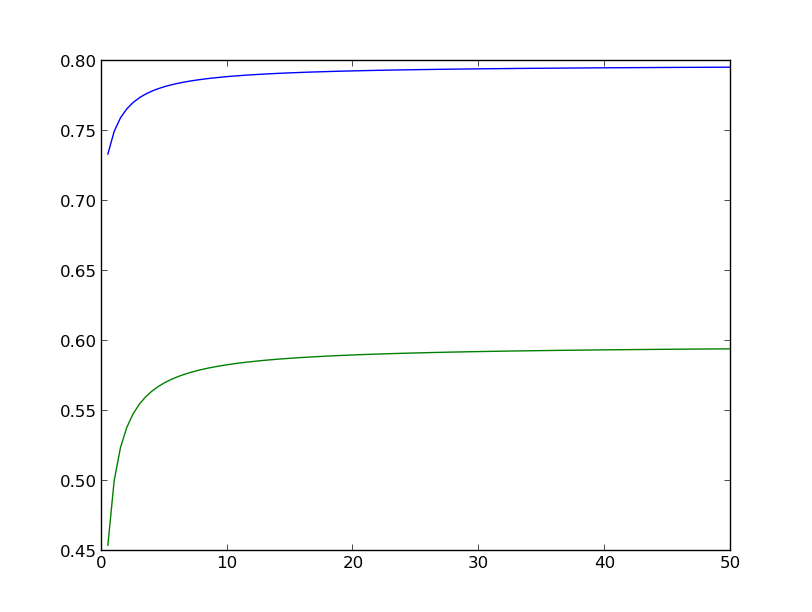
\includegraphics[width=0.6\linewidth,angle=0]{p3.png}
\caption{Octahedron changing resistor}
\label{figure4}
\end{center}
\end{figure}




\newpage
\newpage
(b)
With the linear transformation:
$$
  \begin{cases}
   y_1=x_1+x_5\\
   y_2=x_2+x_4\\
   y_3=x_3\\
   y_4=x_2-x_4\\
   y_5=x_1-x_5\\
     \end{cases}
$$
We have:
\[
  \begin{cases}
	M\ddot{y_1}=-K_{co}y_1+K_{co}y_2\\
	m\ddot{y_2}=K_{co}y_1-(K_{co}+K_{cc})y_2+2K_{cc}y_3\\
	m\ddot{y_3}=K_{cc}y_2-2K_{cc}y_3\\
	m\ddot{y_4}=-(K_{co}+K_{cc})y_4+K_{co}y_5\\
	M\ddot{y_5}=K_{co}y_4-K_{co}y_5\\
  \end{cases}
\]
Then, the matrix equation becomes:


$$
\begin{pmatrix}
 -K_{co} & K_{co} & 0 & 0 & 0 \\
 K_{co} & -(K_{co}+K_{cc}) & K_{cc} & 0 & 0 \\
 0 & K_{cc} & -2K_{cc} & 0 & 0 \\
 0 & 0 & 0 & -(K_{co}+K_{cc}) & K_{co} \\
 0 & 0 & 0 & K_{co} & -K_{co} 
\end{pmatrix}
\begin{pmatrix}
 y_1\\
 y_2\\
 y_3\\
 y_4\\
 y_5
\end{pmatrix}
=
\begin{pmatrix}
 M & 0 & 0 & 0 & 0\\
 0 & m & 0 & 0 & 0\\
 0 & 0 & m & 0 & 0\\
 0 & 0 & 0 & m & 0\\
 0 & 0 & 0 & 0 & M
\end{pmatrix}
\begin{pmatrix}
 \ddot{y_1}\\
 \ddot{y_2}\\
 \ddot{y_3}\\
 \ddot{y_4}\\
 \ddot{y_5}
\end{pmatrix}
$$
with $\omega$:
$$
\begin{pmatrix}
 K_{co} & -K_{co} & 0 & 0 & 0 \\
 -K_{co} & (K_{co}+K_{cc}) & -K_{cc} & 0 & 0 \\
 0 & -K_{cc} & 2K_{cc} & 0 & 0 \\
 0 & 0 & 0 & (K_{co}+K_{cc}) & -K_{co} \\
 0 & 0 & 0 & -K_{co} & K_{co} 
\end{pmatrix}
\begin{pmatrix}
 y_1\\
 y_2\\
 y_3\\
 y_4\\
 y_5
\end{pmatrix}
=\omega^2
\begin{pmatrix}
 M & 0 & 0 & 0 & 0\\
 0 & m & 0 & 0 & 0\\
 0 & 0 & m & 0 & 0\\
 0 & 0 & 0 & m & 0\\
 0 & 0 & 0 & 0 & M
\end{pmatrix}
\begin{pmatrix}
 y_1\\
 y_2\\
 y_3\\
 y_4\\
 y_5
\end{pmatrix}
$$
Thus the eigenvalue can be easily calculated:
$$
\omega^2=\frac{K_{co}}{M}\\
\omega^2=\frac{2K_{cc}}{m}\\
\omega^2=\frac{K_{co}+K_{cc}}{m}\\
\omega^2=0
$$

Sorry, I don't have time to finish this, but I guess you can see I know how to do.
\newpage
\section*{Acknowledgements}

I discussed this assignment with my classmates and used material from the
cited references, but this writeup is my own.

\begin{thebibliography}{9}


\bibitem{coursepage}
PHY 410-505 Webpage, \url{http://www.physics.buffalo.edu/phy410-505}.



\bibitem{bond}
bond strength
\url{http://tieba.baidu.com/p/2670441522}

\bibitem{cs}
bond strength
\url{http://en.wikipedia.org/wiki/Carbon_suboxide}

\end{thebibliography}

\newpage
\appendix
\section{Appendix}

\subsection{python code}

The following python code was used to obtain the results in this report:

\lstinputlisting[language=python]{cube.py}

\lstinputlisting[language=python]{triatomic.py}

\end{document}
